\chapter{Advance Genie Editor}
    \label{chp:genieeditor}

    This is a small guide to \genie{} software. The guide is based on version 2020.3.30. You should not consider this guide as something as official. \genie{} is a program for editing data of genie (\acrref{DAT} and \acrref{DLL}) files. It can edit properties of units, civilizations, technologies, graphics, terrains, sounds, player colors and some other things\cite{TurnupHyperion4:2019}.
    \genie{} program can be found in \aoeexedir{}, under \dquote{Tools\_Build} directory.

    When you execute it three windows automatically open. The \textit{Open files...} allows you to open a \genie{} file. To manage \aoe{} files, click on the button \textit{Age of Empires II: Definitive Edition} on the right of \textit{Defaults:} label. Set the \textit{Genie version:} to \textit{Age of Empires II: Definitive Edition}.
    The file that you need to open is the one specified by \textit{Compressed data set (*.dat)}: such a file should be called \code{empires2\_x2\_p1.dat}. When you open such a file you can view all the unit, buildings, civilizations parameters and properties. The vanilla file is \code{C:\textbackslash{}Program Files (x86)\textbackslash{}Steam\textbackslash{}steamapps\textbackslash{}common\textbackslash{}AoE2DE\textbackslash{}resources\_common\textbackslash{}dat\textbackslash{}empires2\_x2\_p1.dat}.

    After opening the file, you can now make changes on the file. \figref{fig:genie01} shows the state fo the program when it opens the file. 

    \begin{figure}[ht]
        \centering
        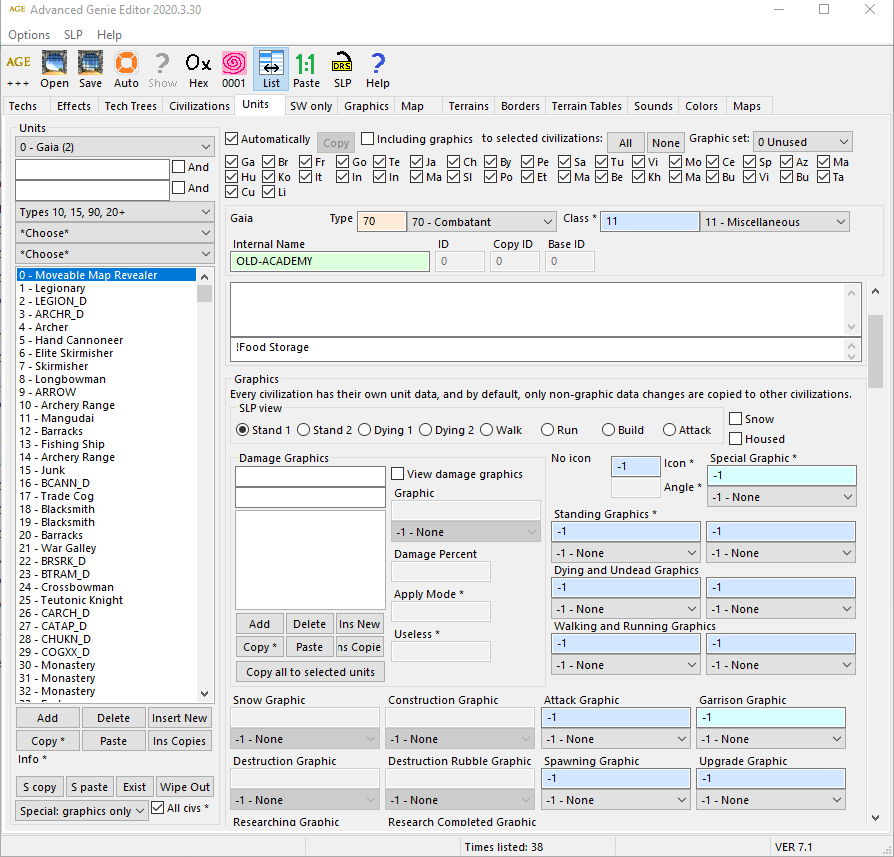
\includegraphics[width=0.7\textwidth]{src/images/genie01}
        \caption{Standard \genie{} window}
        \label{fig:genie01}
    \end{figure}

    As shown in \figref{fig:genie03}, \genie{} splits its parameters regarding the \aoe{} field.

    \begin{info}
        You can switch between tabs by the performing hotkeys \code{Ctrl + Pag. Up} and \code{Ctrl + Pag. Down}.
    \end{info}

    \begin{figure}[ht]
        \centering
        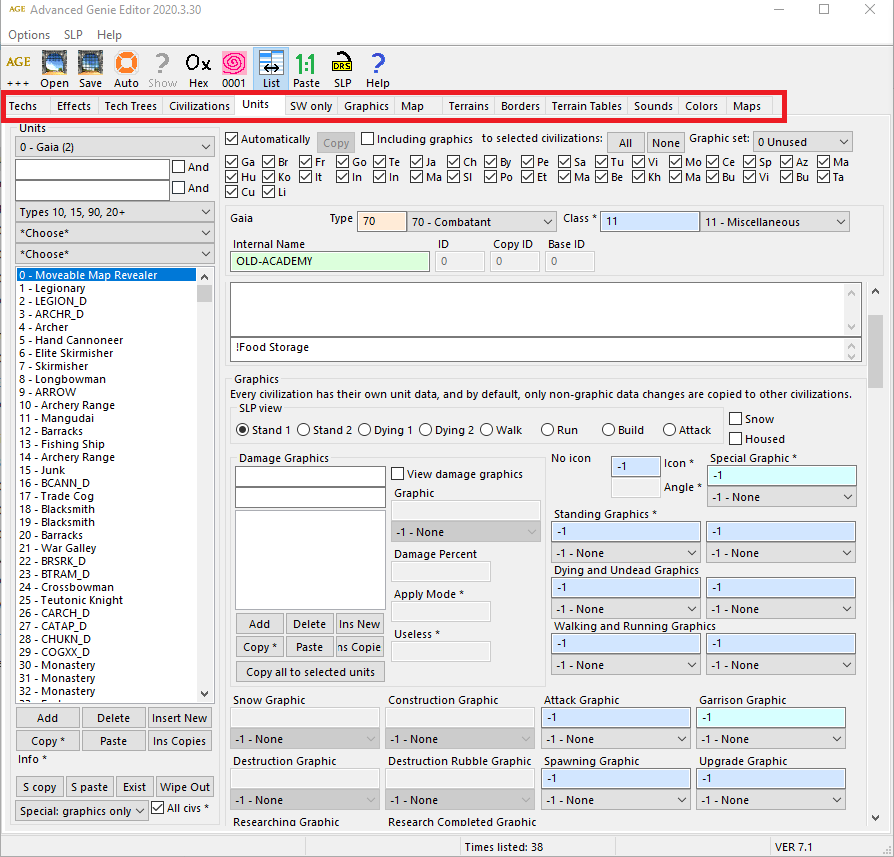
\includegraphics[width=0.7\textwidth]{src/images/genie03}
        \caption{Standard \genie{} window. The red box highlights the category tabs grouping the parameters you can tweak according to the \aoe{} field.}
        \label{fig:genie03}
    \end{figure}

    In the units left pane (called \dquote{Units}) there is displayed the list of all the units a particular civilization can manage (\eg{} in \figref{fig:genie02} the civ is \dquote{Gaia}). Since the unit tabs show several parameters and unit, you can filter the units using the search box in the units pane (\eg{} \figref{fig:genie02} highlighted in the red box).

    \begin{figure}[ht]
        \centering
        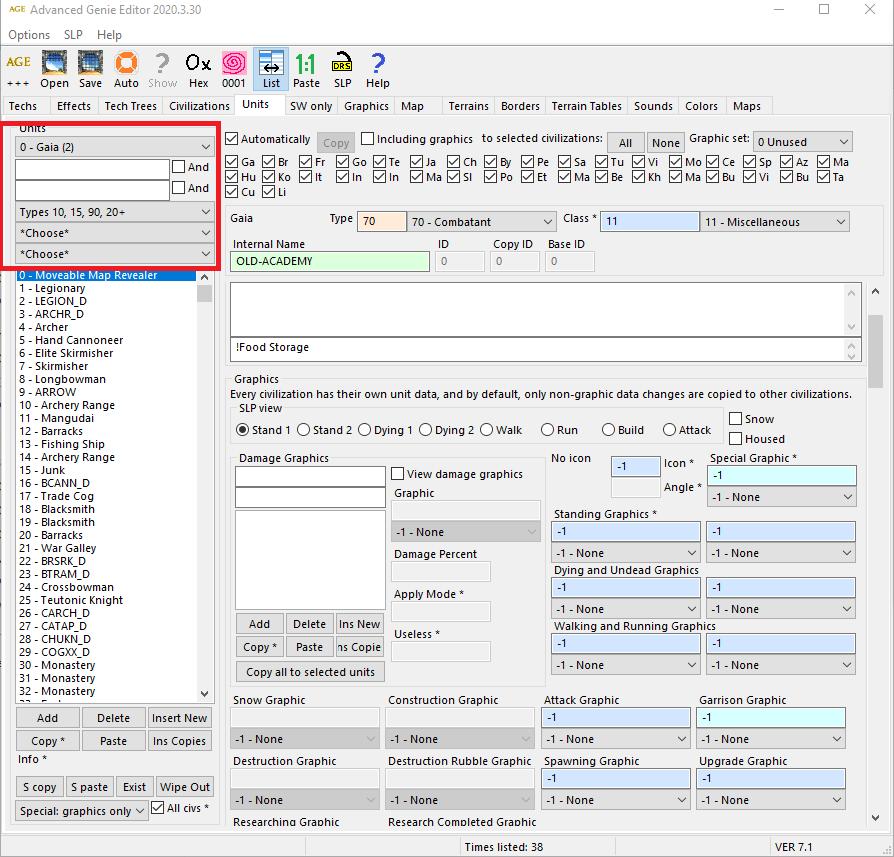
\includegraphics[width=0.7\textwidth]{src/images/genie02}
        \caption{Standard \genie{} window. The red box highlights the search boxes you can use to filter }
        \label{fig:genie02}
    \end{figure}

    The search box works as follows: first you select the civilization, then you can add at most 2 criteria involving the unit name (in and with the civilization): namely, if the 2 criteria are $\gamma_1$ and $\gamma_2$ and the civilization involved is $c$, the whole search criterion is $civ = c \land (\gamma_1 \in unit.name) \land (\gamma_2 \in unit.name)$, where $unit.name$ is the string representing a generic unit name. For instance, if $\gamma_{1} = dead$ then we select all the units whose name contains the substring \dquote{dead}. You can add \dquote{|} to perform a logical or ($\squote{\lor}$) inside $\gamma_{i}$ ($i \in \{1,2\}$). For instance if $\gamma_{1} = \_D|dead$, the global search criterion is $civ = c \land ((\_D \in unit.name) \lor (dead \in unit.name))$: such a search query will generate all the units whose name contains either \dquote{\_D} or \dquote{dead}.

    You can select multiple units: when you alter a value from the unit pane, the same parameter will be updated also in every other civilization checked in the top checkboxes (\eg{}, \dquote{Ga}, \dquote{Br}, \dquote{Fr}, \dquote{Go}). At the bottom you can see how many changes performed in this session (as shown in \figref{fig:bottombar}).

    \begin{figure}[ht]
        \centering
        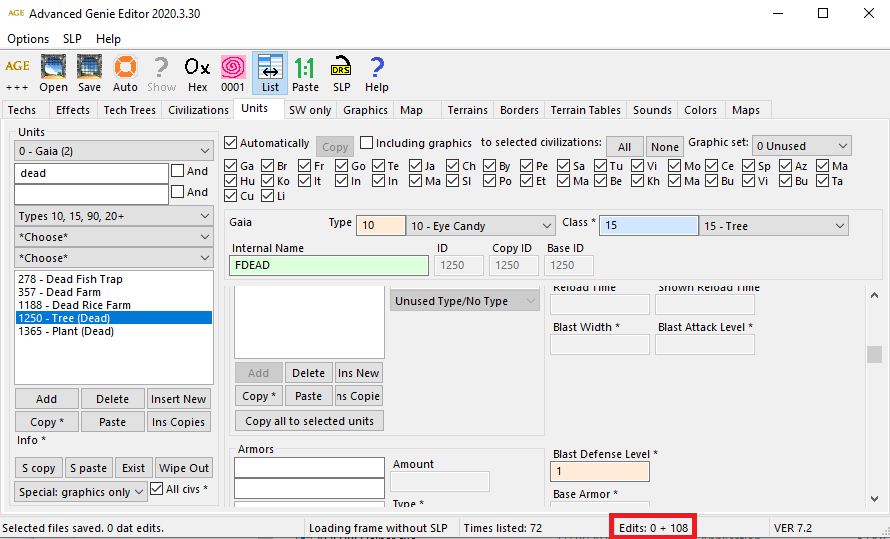
\includegraphics[width=0.8\textwidth]{src/images/bottom-bar}
        \caption{Example of how the bottom bar can be used to check how many changes we have made so far.}
        \label{fig:bottombar}
    \end{figure}

    \section{Required Knowledge}

    \paragraph{Unit names.}
    The units ending with \dquote{\_D} represent the corpses of the associated unit: for instance \dquote{Archer} unit is the actual unit with all its properties while \dquote{ARCHR\_D} represents the archer corpse.

    \paragraph{Buildings.} Every time the user access to a new era, each building changes. For instance, in \textit{graphics} you can see that there are, for each stable building civ, a stable for feudal, one for the castle age and another one for the imperial age.

    \section{Units parameters}

    Manage a single unit parameters. This section is divided in multiple sub areas:

    \begin{itemize}
        \item Language Files;
        \item Graphics;
        \item Statistics;
        \item Projectiles;
        \item Attributes;
        \item Sounds;
        \item Tasks;
    \end{itemize}

    The documentation in this area has been copied from \cite{agewiki:2014}.

    \subsection{Language Files}

    \subsection{Graphics}

    \subsection{Statistics}

    \textbf{Hit Points}: hit points of the unit. If -1, the unit will immediately die\cite{genie:hitpoints}. \textbf{Speed}: the speed of the unit. \textbf{Rotation Speed} makes the unit slower. \textbf{Line of Sight} represents the number of cells the unit can see. Generates a circle centered in the unit. \textbf{Search Radius} is determines the area within which the unit will recognizes and react to other units.  If anything enters this area, the unit will notice it; If you enter a value higher than LOS, a unit will chase enemy units outside of its sight range. \textbf{Min Range} (\textbf{max Range}) represents the minimum (maximum) range the ranged unit can shoot its projectile: for example an archer can shoot any target between 0 and 4 cells\cite{agewiki:2014}.

    \textbf{Resource capacity} determines the quantity of resources a unit can hold (in range $[0, 3392]$): for villagers, this is the max amount of resources they can carry. For other units, it can be other resources, like the time it takes for a dead unit to decompose\cite{agewiki:2014}.

    \textbf{Resource Decay} determines how fast objects (like corpses) decay. Set -1 for never decaying. A negative value will prevent the corpse from decaying permanently. The larger a positive value is, the longer the corpse will last. (The value is approximately the equivalent number of game seconds). Many non-corpse units have resource decay value, but the purpose of it in other units is unknown\cite{agewiki:2014}. 

    \textbf{Work Rate} determines the base work speed of units. This affects rates like villager work rates (building, gathering, etc.), conversion speed, and trebuchet pack (unpack) speed. the value needs to satisfy the constraint $x \geq 0$\cite{agewiki:2014}.

    \textbf{Garrison Capacity} is the number of units a transport or building can hold. allowed value $x$ must satisfy the constraint $x \in [-1, 127]$. Only rams, buildings, and transport ships can normally hold units. \footnote{Garrisoning infantry into rams will increase both the ram's speed and attack.} If you give a rams an original speed of 0, garrisoning units will allow it to move. 

    \textbf{Garrison type} determines what units can garrison into the building ($x \in [0, 15]$). Such a integer value should be interpreted as an enumeration, which semantic is shown in \tblref{tbl:garrisontype}. The number are encoded in \genie{} as a 8-bit value\cite{agewiki:2014}.

    \begin{table}[ht]
        \centering
        \begin{tabular}{ll}
            \toprule
            Value & Semantic \\
            \midrule
            0   &   None \\
            1  &  Villagers only \\
            2  &  Infantry only \\
            3  &  Villagers and infantry \\
            4  &  Cavalry \\
            5  &  Cavalry and villagers \\
            6  &  Cavalry and infantry \\
            7  &  Cavalry, infantry and villagers \\
            8  &  Monks only \\
            9  &  Monks and villagers \\
            10  &  Monks and infantry \\
            11  &  Monks, infantry and villagers \\
            12  &  Monks and cavalry \\
            13  &  Monks, villagers and cavalry \\
            14  &  Monks, cavalry and infantry \\
            15  &  Monks, villagers, infantry and cavalry \\
            \bottomrule
        \end{tabular}
        \caption{Semantic of each Garrison Type value.}
        \label{tbl:garrisontype}
    \end{table}

    \textbf{Garrison Heal Rate} determines how fast a building heals units garrisoned within it ($x \geq 0$). This is different from the Garrison Recovery, which determines how fast the unit heals when garrisoned in any building\cite{agewiki:2014}.

    \subsection{Projectiles}

    \subsection{Attributes}

    \textbf{Dead Unit} Represents the unit representing the corpse of the unit currently under analysis. By convention, all \dquote{dead units} ends with \code{\_D}. If a unit does not have any dead unit, this field is set to $-1$. For example, the dead unit of the unit \dquote{Archer} is set to be \code{ARCHR\_D} unit.

    \subsection{Sounds}

    \subsection{Tasks}

    \section{Graphics}

    Represents the graphics and the animations involved in every units and buildings. This section has been copied from \cite{agewiki:grpahics:2014}. The left pane represents the sprites of each unit, building and so on. There is a search box that is similar to the one in \dquote{Units}.

    \textbf{Internal Name} is the name used to identify the sprites in the \genie{} in the left pane of \dquote{Graphics} panel.

    \textbf{Frames per Angle} represents the framerate of the sprite.

    \textbf{Animation Duration} represents how long the animation is displayed in seconds. After that time the animation stops and the sprite is removed. It is required that $x > 0$. Exponential notation can be used (\eg{} $e3+35$). Use this field if you want to avoid the sinking of dead units for every sprite whose name contains \dquote{(Decay)} substring. If the duration input is larger than the actual animation length, 

    \subsection{Deltas}

    The deltas section allows to combine multiple sprites togther ina single animation. The sprites and animation that are combined are the one shown in the left pane (see \figref{fig:deltas}).

    \begin{figure}[ht]
        \centering
        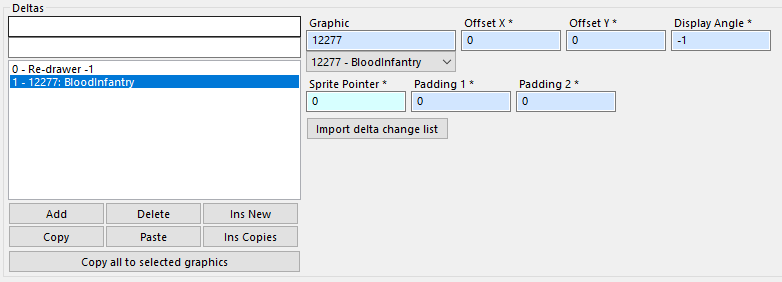
\includegraphics[width=1.0\textwidth]{src/images/deltas}
        \caption{Section of Graphics allowing you to combine different textures together.}
        \label{fig:deltas}
    \end{figure}

    \textbf{Graphic} represents the id of the sprite to show. The name of the file refers to the json file present in \code{resources/\_common/particles}.

    \textbf{Padding 1} and \textbf{Padding 2} are not useful.

    \subsection{Angle Sounds}

    
    %On the top _D|dead \cite{gagmanAoC:2017}